\documentclass[a4paper,10pt]{article}
\usepackage{fullpage}
\usepackage{float}
\usepackage[english]{babel}
\usepackage{graphicx,subfig,wrapfig}
\usepackage{amsmath,amsfonts,amsthm,amssymb}
\usepackage{fancyhdr,fancybox,color}
\usepackage{enumerate}
\usepackage[amssymb]{SIunits}
\definecolor{MyBlue}{rgb}{0,0.3,0.6}
\usepackage[colorlinks=true,
            linkcolor=MyBlue,
            plainpages=false,
            citecolor=MyBlue,
            urlcolor=MyBlue]{hyperref}
\usepackage[all]{hypcap}
\usepackage[url=false,
backend=bibtex,
style=authoryear-comp,
doi=true,
isbn=true,
backref=false,
dashed=false,
maxcitenames=2,
maxbibnames=99,
natbib=true]{biblatex}
\addbibresource{refrence.bib}
\nonfrenchspacing
\begin{document}
\noindent Chair: Physics of Fluids group
\begin{center}
 \begin{LARGE}
  Playing ping-pong with liquid droplets
 \end{LARGE}
\end{center}
\section*{Description}
Recently, during one of his trips to the International Space Station, astronaut Scott Kelly demonstrated that one could play ping-pong in space using water drops (\href{https://www.youtube.com/watch?v=TLbhrMCM4_0}{link here}). This demonstration follows from a long history of research on bouncing drops on superhydrophobic surfaces (see the discussions related to bouncing off superhydrophobic surfaces in \citet{josserand2016drop}).\\
In this study, we would like to understand this process of bouncing droplets. A typical sequence of events is shown in Figure~\ref{Figure::Typical}. In our simulation, we will use an in-house developed read-to-use code to solve the problem of the liquid drop impact on dry substrate. We will focus on the hydrodynamics of the process. In particular, we wish to understand various mechanisms through which the initial kinetic energy of the drop is dissipated in the system.
\begin{figure}[H]
\begin{center}
 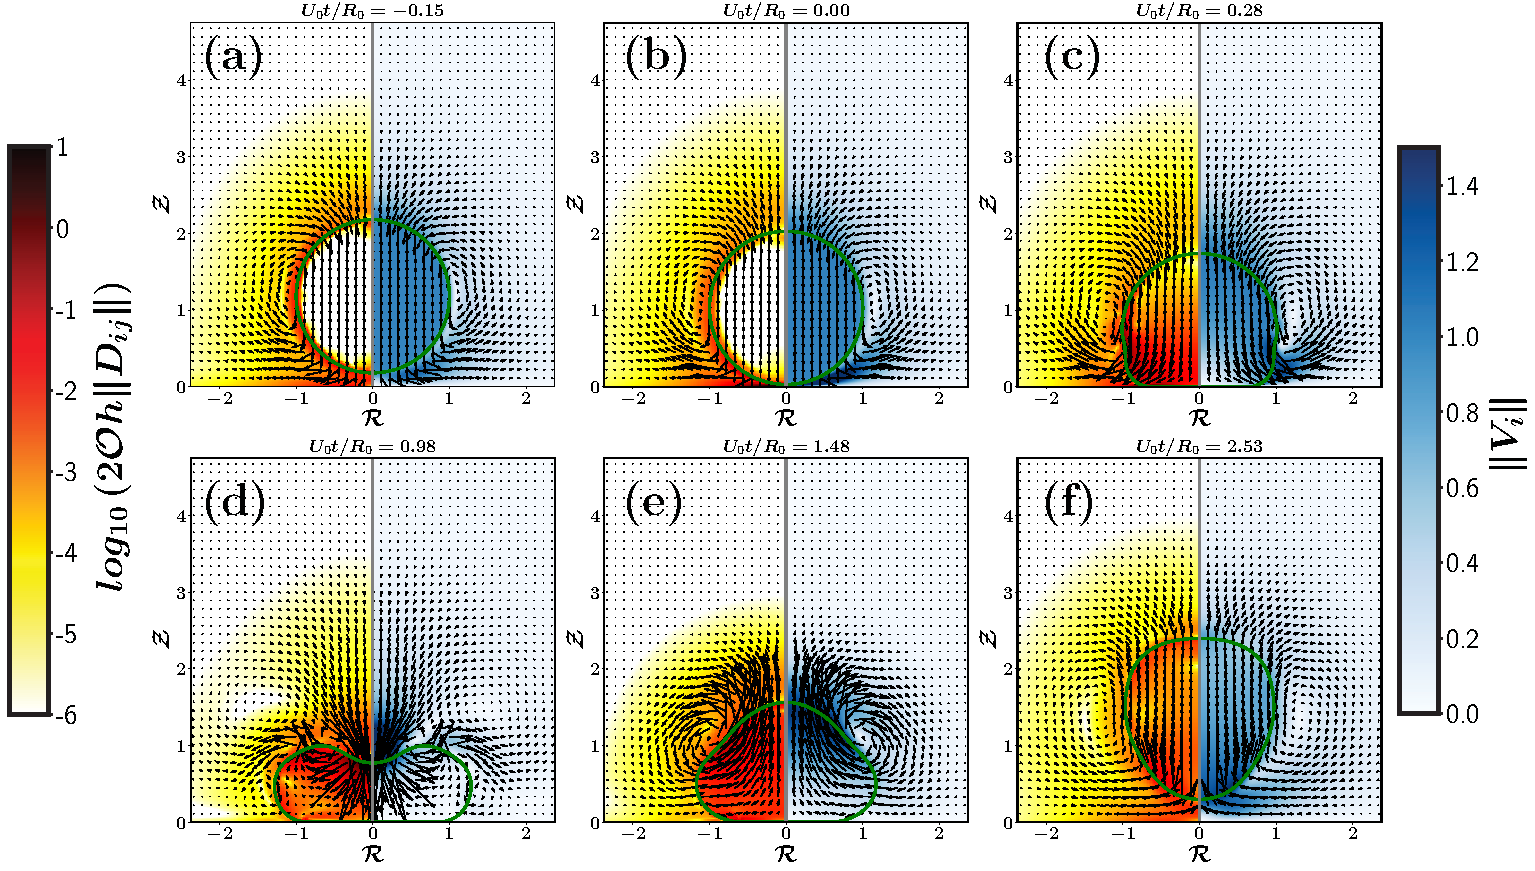
\includegraphics[width=\textwidth]{Figure1.pdf}
 \caption{A typical simulation of a drop bouncing off a superhydrophobic substrate: (a) The drop approaches the substrate, (b) Air is squeezed out of the thin gap between the drop and the substrate, leading to lubrication flow in the gap, (c) The drop spreads on the substrate (see \citet{wildeman2016spreading}), (d) - (e) The drop changes the direction of motion because of the substrate, and (f) The drop bounces back.}
 \label{Figure::Typical}
\end{center}
\end{figure}
\section*{What you will do and what you will learn?}
In the Physics of Fluids group, we are looking for enthusiastic students to work on this topic.
\begin{enumerate}
\itemsep0em
\item You will learn about fundamental fluid dynamics.
\item You will get hands-on experience with Computational Fluid Dynamics (CFD).
\item You will learn how to do basic and advance data analysis.
\end{enumerate}
If you have any questions, fell free to contact \href{mailto:v.sanjay@utwente.nl}{Vatsal} (details below).
\begin{center}
\begin{tabular}{|l|l|l|}
\hline \textbf{Supervision} & \textbf{E-mail} & \textbf{Office} \\
\hline Vatsal Sanjay & \href{mailto:v.sanjay@utwente.nl}{v.sanjay@utwente.nl} & Meander 246B \\
\hline Srinath Lakshman   & \href{mailto:s.lakshman@utwente.nl}{s.lakshman@utwente.nl}& Meander 246A \\
\hline Dr. Pierre Chantelot   & \href{mailto:p.r.a.chantelot@utwente.nl}{p.r.a.chantelot@utwente.nl}& Meander 246B \\
\hline Prof. Detlef Lohse & \href{mailto:d.lohse@utwente.nl}{d.lohse@utwente.nl} & Meander 261  \\
\hline
\end{tabular}
\end{center}
\printbibliography
\end{document}
